\begin{tikzpicture}[align=center]

    \node[inner sep=2.4mm, draw, circle, fill=white!80!blue] 
    (user) {``User''\\Model};
    \node[inner sep=0pt, anchor=center, left=4em of user] 
    (trace) {
\includegraphics[height=.12\textheight]{img/floppy.png}\\Trace};

    \node [inner sep=0pt, anchor=center, right=8em of user] 
    (server) {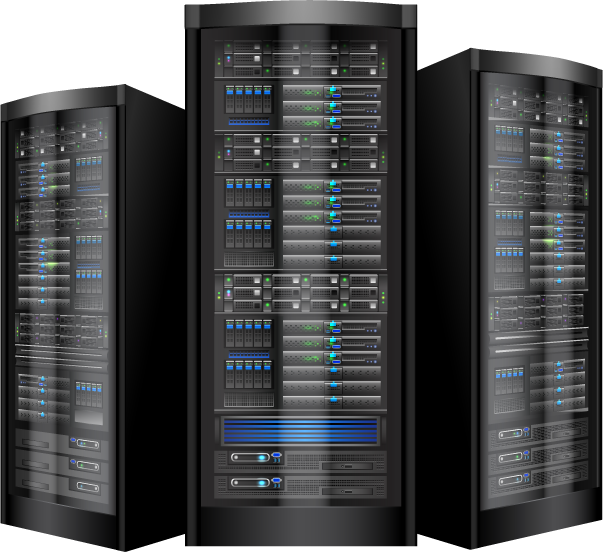
\includegraphics[height=.2\textheight]{img/server.png}};
    
    \coordinate[below=3em of server] (serverarrowanchor) {};

    \draw[very thick, line cap=round, -{Latex[length=2.5mm]}] 
    (user.east) -- coordinate[midway, above] (inputlabelcoord) (server.west);

    \draw[very thick, line cap=round, -{Latex[length=2.5mm]}]
    (trace.east) -- (user.west);

    \draw[very thick, line cap=round]
    (server.south) -- (serverarrowanchor);

    \draw[very thick, line cap=round, -{Latex[length=2.5mm]}]
    (serverarrowanchor) -| (user.south);

    \node[inner sep=0pt, anchor=base, above=1mm of inputlabelcoord] (inputlabel) {Inputs};
    \node[inner sep=0pt, anchor=base, below=18mm of inputlabel] (feedbacklabel) {Feedback};

    \node[fit=(server) (feedbacklabel) (serverarrowanchor), draw, rectangle, dashed, inner sep=1em] (fitbackend) {};
    \node[inner sep=0mm, anchor=base, above=2mm of fitbackend.north] (fitbackendlabel) {Real backend \& network};

    \node[fit=(trace) (user) (user.south |- serverarrowanchor), draw, rectangle, dashed, inner sep=1em] (fituser) {};
    \node[inner sep=0mm, anchor=base, above=2mm of fituser.north] (fituserlabel) {Emulated user};

\end{tikzpicture}